\documentclass[10pt,a4paper]{article}

%double si on veut une version prof et une version élève. simple si on veut une seule version.
\newcommand{\buildmode}{simple}

\InputIfFileExists{version.tex}{}{}
% Version (définie par le script)
\providecommand{\version}{eleve}

\usepackage{feuillecorrection}

%%%à modifier à chaque fois

\renewcommand{\niveau}{1G}
\renewcommand{\chapitre}{Fonctions, généralités}
\renewcommand{\numchap}{0}
\renewcommand{\theme}{Fonctions}

\begin{document}

\begin{multicols}{2}

\begin{corr}{8}


\textbf{a) \(f(x)=4x-3\)}

\smallskip

\textit{Méthode 1 (par le calcul).}
\[
\begin{aligned}
f(x) &\geq 0\\
4x-3 &\geq 0\\
4x-3\textcolor{teal}{+3} &\geq 0\textcolor{teal}{+3}\\
4x &\geq 3\\
4x\textcolor{teal}{\div 4} &\geq 3\textcolor{teal}{\div 4}\\
x &\geq \frac{3}{4}
\end{aligned}
\]
(on divise par \(4>0\), l'inégalité conserve son sens).

\smallskip

\textit{Méthode 2 (graphique).}

\begin{center}
\begin{tikzpicture}[scale=0.9]
\draw[->] (-1.8,0) -- (1.8,0);
\draw[->] (0,-1.8) -- (0,1.8);
\draw[thick,blue] (-1.3,-1.64) -- (1.3,0.44);
\filldraw (0,-0.6) circle (1.3pt);
\node[right] at (0,-0.6) {\scriptsize \(b\)};
\filldraw (0.75,0) circle (1.3pt);
\node[below] at (0.75,0) {\scriptsize \(\frac{3}{4}\)};
\end{tikzpicture}

\(a=4>0 \qquad b=-3<0\)
\end{center}

\begin{center}
\begin{tikzpicture}
\tkzTabInit[lgt=1.1,espcl=1.3]{\(x\) /1, \(f(x)\) /1}{\(-\infty\),\(\frac{3}{4}\),\(+\infty\)}
\tkzTabLine{,-,0,+,}
\end{tikzpicture}
\end{center}

\bigskip

\textbf{b) \(g(x)=-5x+1\)}

\smallskip

\textit{Méthode 1 (par le calcul).}
\[
\begin{aligned}
g(x) &\geq 0\\
-5x+1 &\geq 0\\
-5x+1\textcolor{teal}{-1} &\geq 0\textcolor{teal}{-1}\\
-5x &\geq -1\\
-5x\textcolor{teal}{\div(-5)} &\geq -1\textcolor{teal}{\div(-5)}\\
x &\leq \frac{1}{5}
\end{aligned}
\]
(on divise par \(-5<0\), l'inégalité change de sens).

\smallskip

\textit{Méthode 2 (graphique).}

\begin{center}
\begin{tikzpicture}[scale=0.9]
\draw[->] (-1.8,0) -- (1.8,0);
\draw[->] (0,-1.8) -- (0,1.8);
\draw[thick,blue] (-1.3,1.64) -- (1.3,-0.44);
\filldraw (0,0.6) circle (1.3pt);
\node[right] at (0,0.6) {\scriptsize \(b\)};
\filldraw (0.75,0) circle (1.3pt);
\node[below] at (0.75,0) {\scriptsize \(\frac{1}{5}\)};
\end{tikzpicture}

\(a=-5<0 \qquad b=1>0\)
\end{center}

\begin{center}
\begin{tikzpicture}
\tkzTabInit[lgt=1.1,espcl=1.3]{\(x\) /1, \(g(x)\) /1}{\(-\infty\),\(\frac{1}{5}\),\(+\infty\)}
\tkzTabLine{,+,0,-,}
\end{tikzpicture}
\end{center}

\bigskip

\textbf{c) \(h(x)=x+4\)}

\smallskip

\textit{Méthode 1 (par le calcul).}
\[
\begin{aligned}
h(x) &\geq 0\\
x+4 &\geq 0\\
x+4\textcolor{teal}{-4} &\geq 0\textcolor{teal}{-4}\\
x &\geq -4
\end{aligned}
\]

\smallskip

\textit{Méthode 2 (graphique).}

\begin{center}
\begin{tikzpicture}[scale=0.9]
\draw[->] (-1.8,0) -- (1.8,0);
\draw[->] (0,-1.8) -- (0,1.8);
\draw[thick,blue] (-1.3,-0.44) -- (1.3,1.64);
\filldraw (0,0.6) circle (1.3pt);
\node[right] at (0,0.6) {\scriptsize \(b\)};
\filldraw (-0.75,0) circle (1.3pt);
\node[below] at (-0.75,0) {\scriptsize \(-4\)};
\end{tikzpicture}

\(a=1>0 \qquad b=4>0\)
\end{center}

\begin{center}
\begin{tikzpicture}
\tkzTabInit[lgt=1.1,espcl=1.3]{\(x\) /1, \(h(x)\) /1}{\(-\infty\),\(-4\),\(+\infty\)}
\tkzTabLine{,-,0,+,}
\end{tikzpicture}
\end{center}

\bigskip

\textbf{d) \(i(x)=-x-2\)}

\smallskip

\textit{Méthode 1 (par le calcul).}
\[
\begin{aligned}
i(x) &\geq 0\\
-x-2 &\geq 0\\
-x-2\textcolor{teal}{+2} &\geq 0\textcolor{teal}{+2}\\
-x &\geq 2\\
-x\textcolor{teal}{\div(-1)} &\geq 2\textcolor{teal}{\div(-1)}\\
x &\leq -2
\end{aligned}
\]
(on divise par \(-1<0\), l'inégalité change de sens).

\smallskip

\textit{Méthode 2 (graphique).}

\begin{center}
\begin{tikzpicture}[scale=0.9]
\draw[->] (-1.8,0) -- (1.8,0);
\draw[->] (0,-1.8) -- (0,1.8);
\draw[thick,blue] (-1.3,0.44) -- (1.3,-1.64);
\filldraw (0,-0.6) circle (1.3pt);
\node[right] at (0,-0.6) {\scriptsize \(b\)};
\filldraw (-0.75,0) circle (1.3pt);
\node[below] at (-0.75,0) {\scriptsize \(-2\)};
\end{tikzpicture}

\(a=-1<0 \qquad b=-2<0\)
\end{center}

\begin{center}
\begin{tikzpicture}
\tkzTabInit[lgt=1.1,espcl=1.3]{\(x\) /1, \(i(x)\) /1}{\(-\infty\),\(-2\),\(+\infty\)}
\tkzTabLine{,+,0,-,}
\end{tikzpicture}
\end{center}

\end{corr}

\columnbreak

\begin{corr}{13}



\textbf{a) \(f(x)=(2x-1)(3x+2)\)}

On pose \(u(x)=2x-1\) et \(v(x)=3x+2\), de sorte que \(f=u\times v\). \(u\) a pour coefficient directeur \(2>0\) et s'annule en \(x=\frac{1}{2}\). \(v\) a pour coefficient directeur \(3>0\) et s'annule en \(x=-\frac{2}{3}\).

\begin{center}
\begin{tikzpicture}
\tkzTabInit[lgt=1.1,espcl=1.3]{\(x\) /1, \(u(x)\) /1, \(v(x)\) /1, \(f(x)\) /1}{\(-\infty\),\(-\frac{2}{3}\),\(\frac{1}{2}\),\(+\infty\)}
\tkzTabLine{,-,,-,0,+,}
\tkzTabLine{,-,0,+,,+,}
\tkzTabLine{,+,0,-,0,+,}
\end{tikzpicture}
\end{center}

\(f\) est strictement négative sur \(\left]-\frac{2}{3};\frac{1}{2}\right[\).

\bigskip

\textbf{b) \(g(x)=(3x+1)(-2x)\)}

On pose \(u(x)=3x+1\) et \(v(x)=-2x\), de sorte que \(g=u\times v\). \(u\) a pour coefficient directeur \(3>0\) et s'annule en \(x=-\frac{1}{3}\). \(v\) a pour coefficient directeur \(-2<0\) et s'annule en \(x=0\).

\begin{center}
\begin{tikzpicture}
\tkzTabInit[lgt=1.1,espcl=1.3]{\(x\) /1, \(u(x)\) /1, \(v(x)\) /1, \(g(x)\) /1}{\(-\infty\),\(-\frac{1}{3}\),\(0\),\(+\infty\)}
\tkzTabLine{,-,0,+,,+,}
\tkzTabLine{,+,,+,0,-,}
\tkzTabLine{,-,0,+,0,-,}
\end{tikzpicture}
\end{center}

\(g\) est strictement négative sur \(\left]-\infty;-\frac{1}{3}\right[\cup\left]0;+\infty\right[\).

\bigskip

\textbf{c) \(h(x)=(-x+4)(5-x)\)}

On pose \(u(x)=-x+4\) et \(v(x)=5-x\), de sorte que \(h=u\times v\). \(u\) a pour coefficient directeur \(-1<0\) et s'annule en \(x=4\). \(v\) a pour coefficient directeur \(-1<0\) et s'annule en \(x=5\).

\begin{center}
\begin{tikzpicture}
\tkzTabInit[lgt=1.1,espcl=1.3]{\(x\) /1, \(u(x)\) /1, \(v(x)\) /1, \(h(x)\) /1}{\(-\infty\),\(4\),\(5\),\(+\infty\)}
\tkzTabLine{,+,0,-,,-,}
\tkzTabLine{,+,,+,0,-,}
\tkzTabLine{,+,0,-,0,+,}
\end{tikzpicture}
\end{center}

\(h\) est strictement négative sur \(\left]4;5\right[\).

\bigskip

\textbf{d) \(i(x)=(5x-1)(5x+1)\)}

On pose \(u(x)=5x-1\) et \(v(x)=5x+1\), de sorte que \(i=u\times v\). \(u\) a pour coefficient directeur \(5>0\) et s'annule en \(x=\frac{1}{5}\). \(v\) a pour coefficient directeur \(5>0\) et s'annule en \(x=-\frac{1}{5}\).

\begin{center}
\begin{tikzpicture}
\tkzTabInit[lgt=1.1,espcl=1.3]{\(x\) /1, \(u(x)\) /1, \(v(x)\) /1, \(i(x)\) /1}{\(-\infty\),\(-\frac{1}{5}\),\(\frac{1}{5}\),\(+\infty\)}
\tkzTabLine{,-,,-,0,+,}
\tkzTabLine{,-,0,+,,+,}
\tkzTabLine{,+,0,-,0,+,}
\end{tikzpicture}
\end{center}

\(i\) est strictement négative sur \(\left]-\frac{1}{5};\frac{1}{5}\right[\).

\end{corr}

\end{multicols}

\end{document}
